\chapter*{Стандартизация шугнанского алфавита: теория и~практика}
\addcontentsline{toc}{chapter}{\textit{М.~Меленченко}. \textbf{Стандартизация шугнанского алфавита: теория и~практика}}
\setcounter{section}{0}
\chaptermark{Стандартизация шугнанского алфавита: теория и практика}
\label{chapter-melen-ortho}

\begin{customauthorname}
Максим Меленченко
\end{customauthorname}

\begin{englishtitle}
\i{Standardization of the Shughni alphabet: Theory and practice\\{\small Maksim Melenchenko}}
\end{englishtitle}

\begin{abstract}
Статья посвящена проблеме стандартизации алфавита для шугнанского языка — животрепещущей теме для шугнанцев Таджикистана. В работе представлен проект стандартизированного шугнанского алфавита, а также практические инструменты и рекомендации для комфортного использования этого алфавита на компьютерах. Я надеюсь, что этот текст окажется полезным для всех, кого интересуют проблемы шугнанской письменности, а в особенности исследователей, издателей и литераторов в Таджикистане.
\end{abstract}

\begin{keywords}
шугнанский язык, памирские языки, письменность, кириллица, Юникод, стандартизация алфавита.
\end{keywords}

\begin{eng-abstract}
The article is devoted to the problem of standardization of the alphabet for the Shughni language, a burning issue for the Shughni people of Tajikistan. Although de facto Shughni has been used in writing for a long time now, it still does not have a stable orthography. One of the reasons for this is not the lack of writing systems, but, on the contrary, the abundance of various options for alphabets created by scholars, book publishers and simply language enthusiasts. Thus, speakers are faced with the task of standardization, and these days special attention in standardization should be paid to the use of the alphabet on electronic devices. In the article, I present a project of a standardized Shughni alphabet, as well as practical tools and recommendations for comfortable use of this alphabet on computers. I hope that this text will be useful for everyone interested in the problems of the Shughni orthography, and especially scholars, publishers and writers in Tajikistan.
\end{eng-abstract}

\begin{eng-keywords}
Shughni, Pamir languages, writing, Cyrillic, Unicode, alphabet standardization.
\end{eng-keywords}

\begin{acknowledgements}
Выражаю сердечную благодарность за помощь в подготовке материала для этой статьи Шаҳло Некушоевой, а также своим коллегам по «памирскому проекту» ВШЭ: Юрию Макарову, Дарье Рыжовой, Александру Сергиенко и Борису Якубсону.
\end{acknowledgements}

\begin{initialprint}
\fullcite{melenchenko2023_alphabet}\end{initialprint}

\label{ortho-intro}

Статья посвящена проблеме стандартизации алфавита для~шугнанского языка~— животрепещущей теме для шугнанцев Таджикистана. Хотя де-факто шугнанский язык уже давно не является бесписьменным, у него всё ещё не сложилось устойчивой орфографии. Одна из причин этого заключается не в отсутствии письменности, а~наоборот, в избытке разнообразных вариантов алфавита, создаваемых учёными, издателями и просто языковыми энтузиастами. Таким образом, перед носителями стоит задача стандартизации, причём в наши дни особое внимание при стандартизации стоит уделить использованию письменности на электронных устройствах. В статье я представляю проект стандартизированного шугнанского алфавита, а также практические инструменты и рекомендации для комфортного использования этого алфавита на компьютерах. Я надеюсь, что этот текст окажется полезным для всех, кого интересуют проблемы шугнанской письменности, а~в~особенности исследователей, издателей и литераторов в Таджикистане.

В \hyperref[ortho-theory]{разделе~1} перечислены важные теоретические положения, связанные с разработкой и стандартизацией шугнанских алфавитов. \hyperref[ortho-choice]{Подраздел~1.1} обсуждает проблему выбора букв, \hyperref[ortho-diversity]{подраздел 1.2}~— разнообразие имеющихся алфавитов для шугнанского, а \hyperref[ortho-phoneme]{подраздел~1.3}~— принцип фонематичности. \hyperref[ortho-practice]{Раздел~2} посвящён стандартизации для~электронных устройств (\hyperref[ortho-standard]{2.1}), описанию предлагаемого мной проекта стандартизации (\hyperref[ortho-project]{2.2}) и использованию различных шрифтов для~шугнанского (\hyperref[ortho-fonts]{2.3}).

\pagebreak[4]

В статье используются некоторые общепринятые в научной литературе условные обозначения. Я обозначаю фонематическую транскрипцию косыми чертами //, а фонетическую транскрипцию квадратными скобками []. Использованная в работе транскрипция шугнанского наследует Международному фонетическому алфавиту (МФА) и заимствована из работы [\hyperref[chapter-makplun-morphon]{Макаров, Плунгян 2023}]\fn{Для данного переиздания транскрипция была обновлена по предстоящей публикации \parencite{makarov_jipa} — \i{прим.~переиздания}.}. Ударение в~транскрипции не указывается. Угловыми скобками <> обозначены буквы и~символы, используемые на письме. К примеру, фонематическая транскрипция слова ‘шугнанский’ в МФА выглядит как /χʊɣnønɪ/, при~этом произносится оно как [χʊɣnøːnɛ], а на письме может быть записано по-разному в зависимости от выбранного алфавита — например, как <хуɣ̌ну̊ни>.

\section{Теория} \label{ortho-theory}

\subsection{Выбор букв} \label{ortho-choice}

Алфавиты, применявшиеся для шугнанского языка в Таджикистане в~разные исторические периоды, являются модифицированными вариантами кириллического или латинского алфавитов; в этой статье речь идёт о кириллице\fn{До установления советской власти шугнанцы спорадически пользовались арабской письменностью; её вариант используется современными шугнанцами в Афганистане. Однако так~как в~наши дни в Таджикистане арабица не в ходу, а по своему устройству она сильно отличается от~кириллицы и латиницы, она не обсуждается в этой статье. Подробнее о шугнанской арабице можно прочесть в работе \parencite[80–88]{parker2023}. В 1930-е~годы для шугнанцев Таджикской ССР была разработана и некоторое время~использовалась латиница, но алфавиты на основе латиницы в современном Таджикистане используются только спорадически. В 2013~году на семинаре «Алифбо» в Москве шугнанские литераторы согласились, что в наши дни шугнанский язык должен использовать письменность именно на основе кириллицы \parencite[104]{edelman2016}.}. В разных проектах шугнанской кириллицы многие буквы имеют такое же фонематическое значение, что~и~в русском языке. К~примеру, во всех её вариантах буква <М~м> используется для~обозначения фонемы /m/. Такое~соответствие фонемы и графемы является тривиальным, и никому из~создателей многочисленных шугнанских алфавитов не придёт в голову использовать эту букву для~другого фонематического значения. Однако в~шугнанском языке есть фонемы, которых нет в русском, и которые, соответственно, нельзя отразить русской версией кириллицы (например, /ø/, как в слове /pønd/ ‘дорога’). Именно в отображении этих фонем и различаются варианты шугнанских алфавитов, предлагаемые разными авторами. Проблема отсутствия букв для определённых фонем при создании модифицированных алфавитов может решаться в~первую очередь (а)~введением новых букв или (б)~переназначением неиспользуемых букв из исходного алфавита \parencite[325]{lupke2011}. Создатели шугнанских алфавитов почти всегда использовали способ (а): к примеру, для~отображения фонемы /ø/ часто используется новая буква «у~с~кружком» <У̊~у̊>, которой нет в русском.

Многие варианты шугнанской кириллицы заимствуют буквы не~только из русского, но и из таджикского алфавита. Это связано с~двумя причинами. Во-первых, таджикский язык является государственным языком Таджикистана, и подавляющее большинство шугнанцев Таджикистана говорит на нём в той или иной степени; при этом таджикский уже имеет устойчивый стандартизированный алфавит. Во-вторых, в таджикском есть некоторые фонемы, которые есть также и~в~шугнанском, но отсутствуют в русском — и для них уже придуманы способы отображения в кириллице (например, <Ғ~ғ> /ʁ/, как в слове /ʁɛv/ ‘рот’). Таким образом, заимствование таджикских букв облегчает задачу подбора букв для~шугнанского алфавита. При этом задача не исчезает насовсем, так как многих фонем шугнанского языка в таджикском всё же нет. Рассмотрим подробнее проблемные места при выборе букв для~шугнанского языка — те фонемы, для которых нет прямых соответствий в русском и~таджикском алфавитах.

\begin{enumerate}[(1)]

  \item В шугнанском 10 гласных фонем, из которых три более краткие в~произношении, а остальные семь — более долгие. Некоторые гласные образуют оппозиции по долготе: /a/–/ɑ/, /ɪ/–/i/, /ʊ/–/u/\fn{Как замечают Макаров и Плунгян [\hyperref[chapter-makplun-morphon]{2023}: 4], «для фонологического описания шугнанского вокализма не обязательно использовать понятие долготы», так как между краткими и долгими гласными есть также противопоставление по ряду, подъёму и напряжённости. В переиздании транскрипция была обновлена по предстоящей публикации \parencite{makarov_jipa}, и в обновлённой версии в фонематической транскрипции долгота не обозначается — \i{прим.~переиздания}.}. В русском алфавите нет букв для двух гласных фонем шугнанского языка: /ɛ/ и /ø/, нет также и оппозиций по долготе. Обычно шугнанские алфавиты следуют логичной практике отражать долготу только для тех долгих гласных, которые имеют пару (/ɑ/, /i/ и~/u/). Например, хотя фонема /ɔ/ фонетически является долгой, она не~противопоставлена краткой фонеме, поэтому в шугнанской кириллице её~можно обозначить стандартной кириллической буквой <О~о>\fn{При этом, например, в рушанском языке ситуация отличается: там имеется противопоставление краткой /ɔ/ и долгой /ɔː/ \parencite[17]{pakhalina1969_pamir}.}. Существует некоторая вариативность в~способах обозначения долготы, но~обычно для этого используется диакритический знак «макрон» (черта сверху): краткая <А~а> /a/ противопоставляется долгой <Ā~ā> /ɑ/. Наиболее проблемная гласная — /ø/. С одной стороны, иногда для неё используют букву <Ӯ~ӯ>, которая имеет такое же фонематическое значение в~таджикском. С другой стороны, в <Ӯ~ӯ> есть та же диакритика «макрон», используемая в~других гласных шугнанского алфавита для~обозначения долготы. Поэтому в большинстве алфавитов буква <Ӯ~ӯ> обозначает долгую гласную /u/, в то время как /ø/ выражается буквой «у~с~кружком» <У̊~у̊>.

  \item Шугнанский язык имеет две заднеязычных (/ɣ/ и /x/) и две увулярных (/ʁ/ и /χ/) щелевых согласных. В русском языке есть только заднеязычные щелевые, а в таджикском — только увулярные. Таким образом, необходимо придумать способы различения противопоставления заднеязычных и увулярных на письме. Большинство кириллических шугнанских письменностей используют таджикские буквы <Ғ~ғ> и <Х~х> для увулярных щелевых. Для отображения на письме заднеязычных щелевых используются либо другие заимствованные буквы, либо буквы для увулярных с добавлением диакритик. Зачастую буквы для~заднеязычных щелевых симметрично используют одну и ту же диакритику, «гачек»: заднеязычные <Ɣ̌~ɣ̌> /ɣ/ и <X̌~x̌> /x/ противопоставляются увулярным <Ɣ~ɣ> /ʁ/ и <Х~х> /χ/.

  \item Межзубные щелевые согласные /ð/ и /θ/ отсутствуют и в русском, и в таджикском языках. В шугнанских алфавитах их обычно обозначают либо греческими буквами «дельта» <Δ~δ> и «тета» <Θ~θ>, либо~кириллическими буквами <Д~д> и <Т~т> с добавлением диакритики (<Д̌~д̌> и <Т̌~т̌>).

  \item В шугнанском языке есть аффрикаты: альвеолярные /d͡z/ и /t͡s/ и~постальвеолярные /d͡ʒ/ и /t͡ʃ/. В русском есть буквы только для глухих аффрикат: <Ц~ц> и <Ч~ч>, в таджикском также есть буква для аффрикаты /d͡ʒ/: <Ҷ~ҷ>. Таким образом, проблема выбора новой буквы остаётся только для аффрикаты /d͡z/. В существующих алфавитах она обычно отображается буквами, визуально похожими на русскую <З~з> (например, её~модификацией с~прямой чертой сверху: <Ӡ~ӡ>) или добавлением к ней диакритик.

\end{enumerate}

Итак, я перечислил главные проблемы, связанные с выбором букв для шугнанского кириллического алфавита. Рассмотрим способы, которыми их решали создатели уже существующих алфавитов\fn{Подробное описание истории шугнанских алфавитов можно найти в работах \parencites{dodikhudoeva2005}{dodykhudoeva2020_ortho}{kalandarov2020_yesterday}{edelman2016}.}.

\subsection{Разнообразие шугнанских алфавитов} \label{ortho-diversity}

Начиная с 1960-х~годов московские лингвисты в своих научных работах обычно пользовались международной «иранистической» транскрипцией на основе латиницы [\cite{edelman1963_transcription}; ср.~\cites{sokolova1953}{zarubin1960}{pakhalina1969_pamir}], а в Душанбе исследователи чаще пользовались кириллической транскрипцией [ср.~\cites{karamshoev1963}{zabonkhoi_pamir1972}{pomirshinosi1975}{bakhtibekov1979}]. Эта кириллическая транскрипция унаследовала некоторые черты от~иранистической латиницы (например, греческие и латинские буквы типа <Θ~θ> /θ/, <W~w> /w/ и использование диакритики «гачек» для~заднеязычных щелевых согласных типа <Х̌~х̌> /x/), а некоторые — от~таджикской кириллицы (например, буквы <Ҷ~ҷ> /d͡ʒ/ и <Ғ~ғ> /ʁ/). С~1980-х годов шугнанские учёные активно участвуют в общественных дискуссиях по поводу письменности. В «научно-популярной» версии «общепамирского» алфавита, подготовленного ими в этот период, вместо греческих и некоторых латинских букв предлагается использовать диакритики (<Т̌~т̌> /θ/, <В̌~в̌> /w/ и другие) \parencite[262–263]{dodykhudoeva2020_ortho}. В~серии публикаций 1991–1992~годов лингвист Додхудо Карамшоев предложил более прагматичный подход к~орфографии. По~его~задумке, шугнанский алфавит должен быть полностью совместим с~таджикской кириллицей и не должен требовать никаких дополнительных символов. Отсутствующие в таджикском фонемы Карамшоев предлагал обозначать не греческими и латинскими буквами или~диакритиками, а~диграфами с~<Ъ~ъ> (<ТЪ~тъ> /θ/, <ВЪ~въ> /w/ и~другие). Такое предложение было связано с~техническими ограничениями печати в~Таджикистане в~начале 1990-х \parencite[103]{edelman2016}.

Таким образом, с начала 1990-х в публичной дискуссии об~обозначении фонем, которых нет в русском и таджикском кириллических алфавитах, закрепились три основных решения: (а)~использовать латинские и греческие буквы из иранистической транскрипции, (б)~использовать диграфы с имеющимися буквами и буквой <Ъ~ъ>, (в)~использовать имеющиеся буквы с диакритическими знаками \parencite[35]{dodikhudoeva2005}. В~Таблице~\ref{tab:ortho1} эти три стратегии показаны на~примере фонем /θ/ и~/w/:

\begin{table}[h]
 \centering
 \caption{Три стратегии решения проблемы недостающих букв}
 \smallskip
 \label{tab:ortho1}
 \begin{tabular}{l|cc} \toprule
 \makecell[l]{решение проблемы\\недостающих букв} & фонема~/θ/ & фонема /w/ \\ \midrule
 \makecell[l]{(а)~греческие\\и~латинские буквы} & <Θ~θ> & <W~w> \\
 (б)~диграфы с <Ъ~ъ> & <ТЪ~тъ> & <ВЪ~въ> \\
 (в)~буквы с~диакритиками & <Т̌~т̌> & <В̌~в̌> \\ \bottomrule
 \end{tabular}
\end{table}

К сожалению, усилия Карамшоева по стандартизации шугнанской кириллицы оказалась не слишком успешны. Шугнаноязычные издания, выходящие с~1990-х и по наши дни в Таджикистане, используют свои модификации алфавитов, которые могут сильно отличаться друг от друга; новые варианты регулярно предлагаются и в наши дни \parencite[21]{edelman2020_steps}. Более того, многие авторы предлагают письменности, в которых вводятся новые символы. При подготовке этой статьи я исследовал алфавиты, используемые в~разных шугнаноязычных публикациях 2000–2010-х~годов, и обнаружил, что как минимум в семи из них для~обозначения некоторых фонем вводятся новые, не использованные в~предыдущих алфавитах символы (см.~Таблицу~\ref{tab:ortho2}).

\begin{table}[h]
 \centering
 \caption{Примеры введения новых символов для шугнанских фонем в~публикациях 2000–2010-х~годов}
 \smallskip
 \label{tab:ortho2}
 \begin{tabular}{cc|l} \toprule
 символ & фонема & публикация \\ \midrule
 <Ҙ~ҙ> & /d͡z/ & перевод Евангелия от Луки \parencite{dodixudoev2001} \\
 <Д̃~д̃> & /ð/ & \makecell[l]{алфавит Богшо Лашкарбекова, созданный\\в~рамках семинара «Алифбо» в 2013~году\\\parencite{lashkarbekov2020}} \\
 <Χ~χ> & /x/ & \multirow{2}{*}{\makecell[l]{«Фолклори Помир», том~II\\\parencite{shakarmamadov2005}}} \\
 <Z~z> & /d͡z/ & ~ \\
 <ẋ> & /x/ & \multirow{2}{*}{\makecell[l]{«Фолклори Помир», том~III\\\parencite{rizvonshoeva2012}}} \\
 <ӌ> & /d͡ʒ/ & ~ \\
 <УО~уо> & /ø/ & \multirow{2}{*}{\makecell[l]{переиздание сборника стихов\\«Гулғунча» Нодира Шанбезоды [\cite*{gulguncha2012}]}} \\
 <ЭЭ~ээ> & /ɛ/ & ~ \\
 <Ð~ð> & /ð/ & \makecell[l]{сборник стихов «Нāн зив»\\Сафо Алиназара [\cite*{alinazar2017}]} \\
 <Ǯ~ǯ> & /d͡z/ & \multirow{2}{*}{\makecell[l]{роман Худобахша~Худобахшова [\cite*{khudobakhshov2017}]\\«Зиндаги аз~наw ца~су̊д сар»}} \\
 <Ѡ~ѡ> & /w/ & ~ \\ \bottomrule
 \end{tabular}
\end{table}

Очевидно, что такое разнообразие вариантов передачи звуков шугнанского языка не способствует образованию стандартизированной письменной традиции. И детям, и взрослым трудно читать и писать на~родном языке, если в каждой второй книге (которых и так немного) для~его записи используются разные символы. Более того, хаотичность алфавитов может проявляться не только в разных публикациях, но~и~внутри одной публикации. Так, в издании сборника стихов «Нāн зив» Сафо Алиназара [\cite*{alinazar2017}] фонема /ð/ обычно выражается буквой <Ð~ð>, но иногда — диграфом <ДЪ~дъ>. Разные буквы для записи одного звука могут появиться даже в соседних строчках — вероятно, по~недосмотру редакторов (см.~Рисунок~\ref{fig:ortho1})\fn{В изначальной версии статьи было указание на проблемы с написанием фонемы /d͡ʒ/, но это замечание оказалось ошибочным и в переиздании было заменено на другое — \i{прим.~переиздания}.}. Другой пример: в~алфавите, предложенном Бахтоваршоевым [\cite*{bakhtovarshoev2013}], в некоторых диграфах для~согласных используется «твёрдый знак» <Ъ~ъ>, а~в~некоторых «мягкий знак» <Ь~ь>. Например, фонему /θ/ предлагается обозначать диграфом <ТЪ~тъ> с «твёрдым знаком», в~то~время как диграф <ВЬ~вь> /w/ использует «мягкий знак». Непонятно, почему автор не~использовал во~всех диграфах только один из~двух символов (например, «твёрдый знак»), что позволило бы убрать из~алфавита одну лишнюю графему.

\begin{figure}[h]
 \centering
 \caption{Фрагмент публикации \parencite[26]{alinazar2017}}
 \smallskip
 \label{fig:ortho1}
 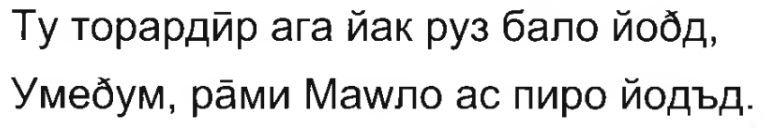
\includegraphics[width=0.6\textwidth]{img/ortho1.jpg}
\end{figure}

Важным фактором принятия решений при стандартизации алфавита является наличие существующей традиции использования \parencites[284]{seifart2008}[6–8]{stark2010}. В Таджикистане издаётся не так много шугнаноязычных книг, и тем не менее, за последние десятилетия накопилось значительное число изданий, которые использовали разные варианты письменности. Следует учитывать их существование и выбирать наиболее консенсусные буквы — такие, которые позволят пользователям стандартизированного алфавита читать эти книги без особых трудностей.

\subsection{Фонематичность и орфография} \label{ortho-phoneme}

Согласно общепринятому мнению, качественный алфавит должен следовать фонематическому принципу, то есть отражать каждую фонему отдельной буквой \parencite[141]{grenoble_whaley2005}. В современном шугнанском языке 29~согласных и 10~гласных фонем [\hyperref[chapter-makplun-morphon]{Макаров, Плунгян 2023}]. Соответственно, качественный шугнанский алфавит должен состоять из 39~букв, каждая из которых однозначно соответствует одной фонеме.

В большинстве предлагаемых алфавитов для шугнанского принцип фонематичности соблюдается, но есть и несколько исключений, связанных с фонетическими особенностями шугнанского. В~современном языке гласные /ɪ/ и /ʊ/ на конце слова произносятся более открыто, то есть как [ɛ] и [o] соответственно (например, /χʊɣnønɪ/ ‘шугнанский’ звучит как [χʊɣnøːnɛ]). Это сравнительно недавняя особенность шугнанской речи: ещё в середине XX~века имела место вариативность, и некоторые носители произносили конечный /ɪ/ как [ɪ], но~в наши дни в Хороге такое произношение уже не встречается [\hyperref[chapter-makplun-morphon]{Макаров, Плунгян 2023}: 11–12; \cite[61–62]{parker2023}]. По~этой причине Додхудо Карамшоев в своей кириллической транскрипции в грамматике баджувского диалекта [\cite*{karamshoev1963}] и~в словаре \parencite{karamshoev1988} отошёл от~принципа фонематичности и~использовал отдельные символы для~«открытого» /ɪ/ и~«открытого» /ʊ/. Например, для союза /ɪdɪ/ ‘что’ в~словаре указаны два~варианта произношения: традиционный <иди> [ɪdɪ] и «открытый» <идę> [ɪdɛ]; во~втором используется специальная буква <ę>\fn{В бумажном издании используется диакритика «точка снизу»; в электронной же версии словаря \parencite{makarov_etal2022} для читабельности используется другая диакритика: <Ę~ę>.}. Бахтоваршоев [\cite*{bakhtovarshoev2013}, \cite*{bakhtovarshoev2016}] также использует отдельный символ для~«открытого» /ɪ/. Он сам признаёт этот «недостаток» и не приводит никаких доводов в пользу отказа от~фонематичности, но замечает, что~«в~действительности этот принцип [фонематичности] в чистом виде нигде полностью не~реализован» (видимо, имеется в виду, что многие языки мира используют нефонематичные алфавиты) \parencite[531]{bakhtovarshoev2013}.

Действительно, фонематический принцип не является универсальным. Во-первых, некоторые алфавиты существуют уже очень долго и были использованы для записи значительного объёма разных текстов, но засчёт исторического изменения фонетики современное произношение слов отличается от их написания. Например, так устроены английский или французский алфавиты. Во-вторых, существуют языки, отличающиеся сложными фонетическими процессами (морфонологические чередования, тоновые различия и прочие). В таких случаях фонематичная запись может отличаться от произношения слишком сильно, и может быть полезно приблизить написание слов к~реальному произношению. Тем не менее, для шугнанского языка эти~аргументы против фонематичной записи неприменимы. Шугнанский не имеет устойчивой письменной традиции (существующие с начала XX~века тексты записаны самыми разными способами), а~его фонетические правила сравнительно просты. Поэтому шугнанский алфавит в идеале должен быть фонематичным — и~большинство предлагаемых вариантов удовлетворяют этому принципу.

В случае шугнанского, помимо общих доводов, актуальны несколько конкретных аргументов в пользу фонематичности. Во-первых, набор фонем шугнанского языка определён достаточно давно \parencite{sokolova1953}, и его корректность с тех пор не подвергалась сомнениям. Это~значит, что создать фонематичный алфавит для шугнанского сравнительно легко — чем~не~могут похвастаться многие языки со~сложной фонетикой. Во-вторых, фонематичная запись отражает историческое произношение и~таким образом сближает шугнанскую орфографию с орфографиями других шугнано-рушанских языков. К~примеру, в бартангском языке, в~отличие от~шугнанского, /ɪ/ не~переходит в [ɛ] на конце слов [О.~И.~Беляев, л.~с.]. Фонематичный алфавит для шугнанского, который отражает более старое обще-шугнано-рушанское произношение конечного /ɪ/, позволит носителям бартангского с большей лёгкостью читать шугнанские тексты (см.~об этой проблеме \parencite[110–111]{edelman2016}; также см.~\parencite[151–153]{grenoble_whaley2005}).

В этой статье я ограничиваюсь обсуждением создания стандартизированной письменности. Между тем, создание письменности~— только один из этапов создания орфографической традиции. Следующим этапом является стандартизация собственно орфографических правил, то есть правил написания конкретных слов, определения границ слов, правил пунктуации и некоторых других \parencites[277]{seifart2008}[322]{lupke2011}[106–107]{edelman2016}. Как пишет Эдельман [\cite*[21–22]{edelman2020_steps}], в~данный момент имеют место только попытки начала разработки орфографических правил (к примеру, в учебнике Аламшоева [\cite*{alamshoev2014}]; см.~также \parencite{edelman2010}).

К примеру, важной орфографической проблемой для шугнанского является написание пресловутого конечного /ɪ/. Эту проблему можно решать двумя способами: (а)~сохранять историческое написание (например, <иди> /ɪdɪ/ ‘что’) или (б)~отражать современное произношение [ɪdɛ]. В большинстве случаев изданные тексты, видимо, следуют первой стратегии и пишут <иди>. Стоит отметить, что второе решение не~обязательно противоречит фонематичности, и для него не обязательно вводить отдельную букву для~«открытого» /ɪ/, как делал Карамшоев. Вместо этого можно, например, использовать здесь букву для фонемы /ɛ/ (например, <идê>) — как я имел возможность наблюдать, при письме носители шугнанского часто делают именно так. Другая важная проблема орфографии касается слитного, дефисного или раздельного написания клитик — например, послелогов (<мāшанд> vs~<мāш-анд> ‘у~нас’) или~союзов (<цачӯд> vs~<ца-чӯд> vs~<ца~чӯд> ‘что сделал:а’). Эти и другие проблемы орфографии предстоит решать уже после утверждения стандартизированного алфавита~— о котором и пойдёт речь в следующем разделе.

\section{Практика} \label{ortho-practice}

\subsection{Стандартизация для электронных устройств} \label{ortho-standard}

Так как для шугнанского языка пока что нет общепринятого стандартизированного алфавита, шугнанская кириллица отсутствует в~каталогах официальных раскладок клавиатуры в Windows, macOS и~на~смартфонах. Соответственно, в~быту носители шугнанского пользуются разнородными и спонтанными практиками электронного письма. Поэтому стандартизация алфавита должна включать в себя в том числе стандартизацию записи букв по~Юникоду — системе кодирования символов, которая используется на~современных электронных устройствах. Юникод представляет из себя систему соответствия символов и кодов, под которыми они хранятся в~памяти компьютеров и телефонов: к~примеру, заглавная кириллическая буква «А» имеет код U+0410.

Важно, что термины «буква» и «символ» здесь не равны друг другу. \b{Буквой} я называю то, как знак выглядит, а \b{символом} — то,~как~он закодирован для электронных устройств. Некоторые буквы в~Юникоде можно закодировать разными символами. К примеру, символы <A> и <А> выглядят для человека как одна и та же буква, но~для~компьютера это два разных символа: слева латинская заглавная «А» (в~Юникоде имеет код~U+0041), справа кириллическая заглавная «А» (код U+0410). Если~воспользоваться автоматическим поиском по тексту (например, в~Microsoft Word), не~получится найти латинскую «А» в тексте, где~используется только кириллическая — потому что автоматический поиск работает с~символами и не обращает внимание на то, насколько они~похожи визуально.

Актуальность этой проблемы конкретно для шугнанского можно проиллюстрировать на следующем примере. Допустим, мы решили, что~фонема /ɣ/ будет обозначаться греческой буквой «гамма». Однако этого недостаточно: в Юникоде можно найти много символов, похожих по~начертанию на «гамму». Это и оригинальная греческая буква «гамма» <Γ~γ>, и так называемая «латинская гамма» <Ɣ~ɣ> (заметьте, как у них отличается начертание заглавной буквы), и кириллическая «у с прямым концом» <Ү~ү> (используемая, например, в казахской кириллице). Аналогичная проблема касается и других букв, для которых есть несколько вариантов кодирования в Юникоде: в частности, букв «тета» (<Θ~θ> vs <ϴ~ϑ>) и~«дзе» (<Ӡ~ӡ> vs <Ʒ~ʒ>). Во многих современных шугнаноязычных книгах используются одни и те же буквы, но разные символы. Таким образом, при стандартизации необходимо выбрать не только начертания, но и конкретные символы \parencite[326–328]{lupke2011}. Без этого невозможно, например, создать раскладку клавиатуры, так как клавиатура компьютера использует именно символы Юникода.

Отсутствие единого стандарта по Юникоду является причиной графической неопрятности многих текстов, изданных на шугнанском языке, в 2000–2010-х годах. Нередко встречается ситуация, когда редакторы, по-видимому, не смогли указать заглавные символы для~некоторых букв. Например, в начале учебника Аламшоева [\cite*{alamshoev2014}] приведён алфавит, используемый в книге, но для четырёх букв в нём не~указан заглавный вариант, а два повторяется строчная буква: <γγ>, <ӡӡ> и так далее (Рисунок~\ref{fig:ortho2}). То же можно увидеть в издании \parencite{alinazar2017}: редакторы не смогли найти заглавный вариант буквы <ẙ> /ø/, поэтому для~заголовка, напечатанного целиком заглавными буквами, им пришлось вставить строчную букву и увеличить ей размер шрифта (Рисунок~\ref{fig:ortho3}).

\begin{figure}[h]
 \centering
 \caption{Алфавит из учебника \parencite{alamshoev2014}}
 \smallskip
 \label{fig:ortho2}
 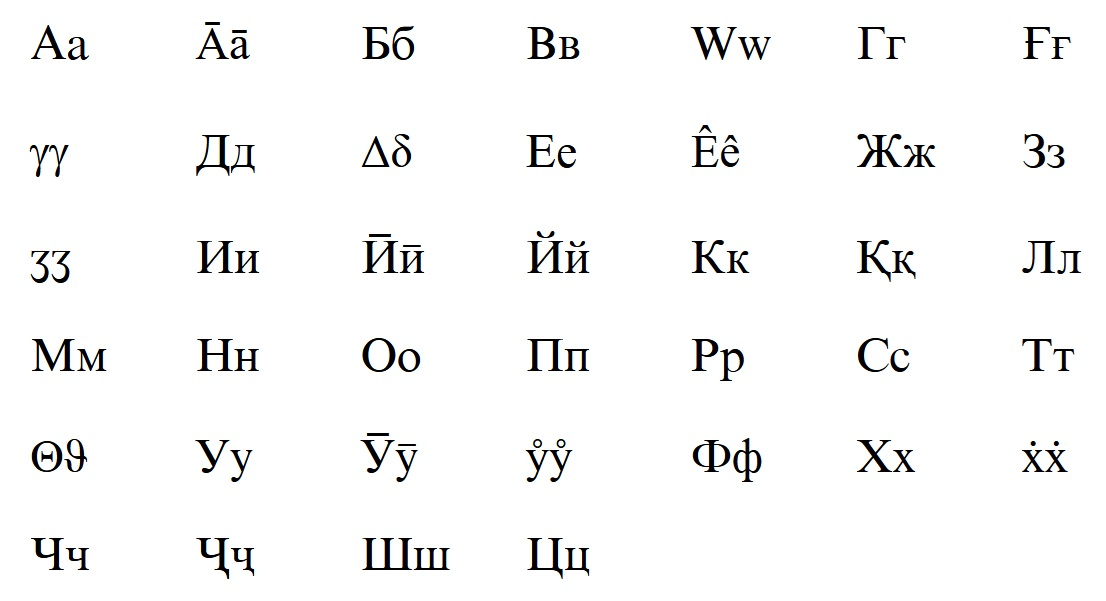
\includegraphics[width=0.8\textwidth]{img/ortho2.jpg}
\end{figure}

\begin{figure}[h]
 \centering
 \caption{Фрагмент публикации \parencite[19]{alinazar2017}}
 \smallskip
 \label{fig:ortho3}
 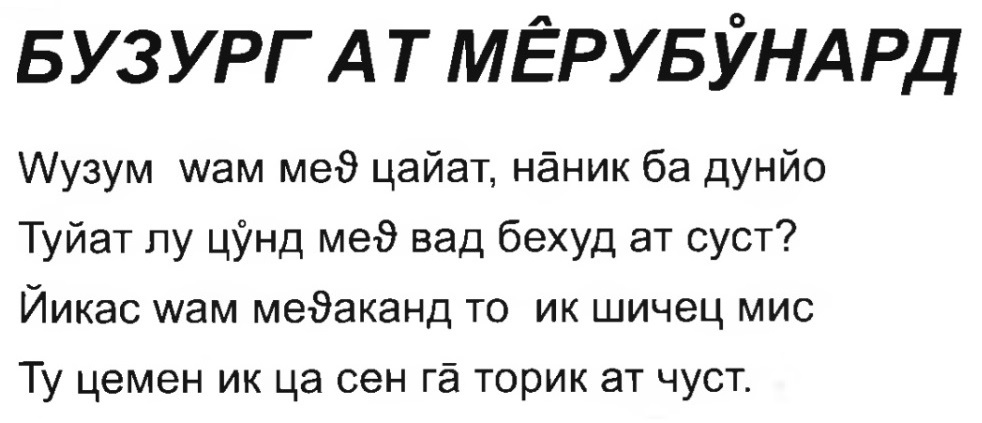
\includegraphics[width=0.6\textwidth]{img/ortho3.jpg}
\end{figure}

\pagebreak[4]

Диакритики представляют особую проблему для отображения на~электронных устройствах. Дело в том, что для многих комбинаций букв и диакритик в~Юникоде есть цельный символ. С другой стороны, любые комбинации букв и диакритик можно ввести с помощью композита, то~есть сначала символ буквы, а потом символ диакритики. С точки зрения в~первом случае использован один символ, а~во~втором~— два. Отличие для~рядового пользователя заключается, например, в том, что если на~компьютере набрать цельный символ, а потом нажать клавишу Backspace, то символ удалится целиком; у~композитной буквы же удалится только диакритика. Если возможно, лучше использовать для алфавита цельные символы (об этом подробнее в~\hyperref[ortho-fonts]{Разделе~2.3}).

\subsection{Стандартизированный алфавит} \label{ortho-project}

В этом разделе я представляю свой проект стандартизации шугнанского алфавита, который основан на консенсусном варианте шугнанской кириллицы. Этот вариант наиболее близок к алфавиту, использовавшемуся в последние годы в детских книгах типа \parencite{rizvonshoeva2015} и названному Д.~Эдельман [\cite*[104]{edelman2016}] «наиболее удачным». Он~не~предлагает никаких кардинально новых решений, а наоборот, использует наиболее распространённые практики для передачи шугнанской фонетики на письме. Он является фонематичным и~содержит 39~букв, соответствующих 39~фонемам шугнанского языка. Ниже я перечислю его основные особенности.

Гласная /ɛ/ обозначается символом <Ê~ê>; гласная /ø/ обозначается символом <У̊ у̊>. Долгота гласных обозначается «макроном», то есть горизонтальной чертой сверху. При этом долгота помечается только у~гласных <Ā~ā> /ɑ/, <Ӣ~ӣ> /i/ и <Ӯ~ӯ> /u/ (об этом см.~в~\hyperref[ortho-choice]{Разделе~1.1}). Для~аффрикаты /d͡z/ используется буква «дзе» <Ӡ~ӡ>, заимствованная из~абхазского алфавита. Также используются два очевидных символа из~таджикской кириллицы: <Қ~қ> /q/ и <Ҷ~ҷ> /d͡ʒ/, и латинская буква <W~w>~/w/.

\pagebreak[2]

Межзубные щелевые согласные /ð/ и /θ/ обозначаются греческими буквами «дельта» <Δ~δ> и «тета» <ϴ~θ>. Увулярные щелевые /ʁ/ и /χ/, как~и~в таджикском, обозначаются буквами <Ғ~ғ> и <Х~х>. Для~заднеязычных щелевых /ɣ/ и /x/ используются буквы «латинская гамма» с~гачеком <Ɣ̌~ɣ̌> и «х» с гачеком <Х̌~х̌>\fn{На мой взгляд, наиболее спорным вопросом здесь является необходимость наличия гачека в~букве <Ɣ̌~ɣ̌> /ɣ/. Изначально я считал, что здесь можно обойтись без гачека, так как, в отличие от~<Х̌~х̌>, в предлагаемом алфавите нет соответствующей буквы без гачека, и таким образом, нет~нужды использовать на гамме диакритику. Однако использование диакритики было поддержано сотрудни:цами Института гуманитарных наук г.~Хорог в личной беседе (2023), поэтому я~включаю в~предлагаемый вариант именно гамму с гачеком <Ɣ̌~ɣ̌>.}.

По возможности я использовал цельные символы Юникода (<Ā~ā>, <Ê~ê> и другие). К сожалению, в Юникоде нет цельных символов для~таких букв, как <У̊~у̊>\fn{В Юникоде есть цельный символ <ẙ> (U+1E99), который можно было бы здесь использовать. Однако у этого символа нет заглавного варианта, поэтому он непригоден для полноценного алфавита.}, <Х̌~х̌> и <Ɣ̌~ɣ̌>, поэтому для них использованы композиты, и в некоторых шрифтах их диакритика может «съезжать» в~сторону. Полный проект стандартизации с соответствиями букв и кодов Юникода можно прочитать в~онлайн-документе \parencite{melenchenko2023_unicode} по~ссылке: \i{\href{https://drive.google.com/file/d/1EafEzbr-vX_Y2g6ax41UcUU3RNzY4f0o}{drive.google.com/file/d/1EafEzbr-vX\_Y2g6ax41UcUU3RNzY4f0o}}. Визуально предлагаемый стандартизированный алфавит выглядит так:

\begin{table}[H]
 \centering
 \label{tab:ortho_alphabet}
 \begin{tabular}{cccccccccc}
 Аа & Āā & Бб & Вв & Ww & Гг & Ғғ & Ɣ̌ɣ̌ & Дд & Δδ \\
 Ее & Êê & Жж & Зз & Ӡӡ & Ии & Ӣӣ & Йй & Кк & Ққ \\
 Лл & Мм & Нн & Оо & Пп & Рр & Сс & Тт & Θθ & Уу \\
 Ӯӯ & У̊у̊ & Фф & Хх & Х̌х̌ & Цц & Чч & Ҷҷ & Шш & ~ \\
 \end{tabular}
\end{table}

Для использования этого алфавита на компьютерах я вместе с~Борисом Якубсоном разработал раскладки для Windows и macOS. Расположение букв в этих раскладках основано на стандартной русской схеме ЙЦУКЕН. Некоторые отсутствующие в русском буквы шугнанского алфавита набираются самостоятельными клавишами, другие~— при~помощи вспомогательной клавиши AltGr. Схема раскладок устроена таким образом, чтобы более частотные буквы имели собственные клавиши и располагались ближе к центру для удобства печати\fn{Данные о частотности букв шугнанского алфавита подсчитаны автоматически на материале текста романа Х.~Худобахшова «Зиндаги аз~наw ца~су̊д сар» [\cite*{khudobakhshov2017}].}. Раскладки адаптированы для профессиональной работы с~текстом: кроме букв и~стандартных символов, в них добавлены дополнительные типографские символы (неразрывный пробел, разные виды тире и кавычек и другие знаки пунктуации), схема расположения которых позаимствована из~кириллической раскладки Ильи Бирмана [\cite*{birman}]. Эти раскладки можно скачать на сайте \i{\href{https://shglayouts.pythonanywhere.com}{shglayouts.pythonanywhere.com}}. К~примеру, схема раскладки для Windows выглядит так:

\begin{figure}[H]
 \centering
 \caption{Схема созданной раскладки с шугнанской кириллицей для Windows}
 \smallskip
 \label{fig:ortho4}
 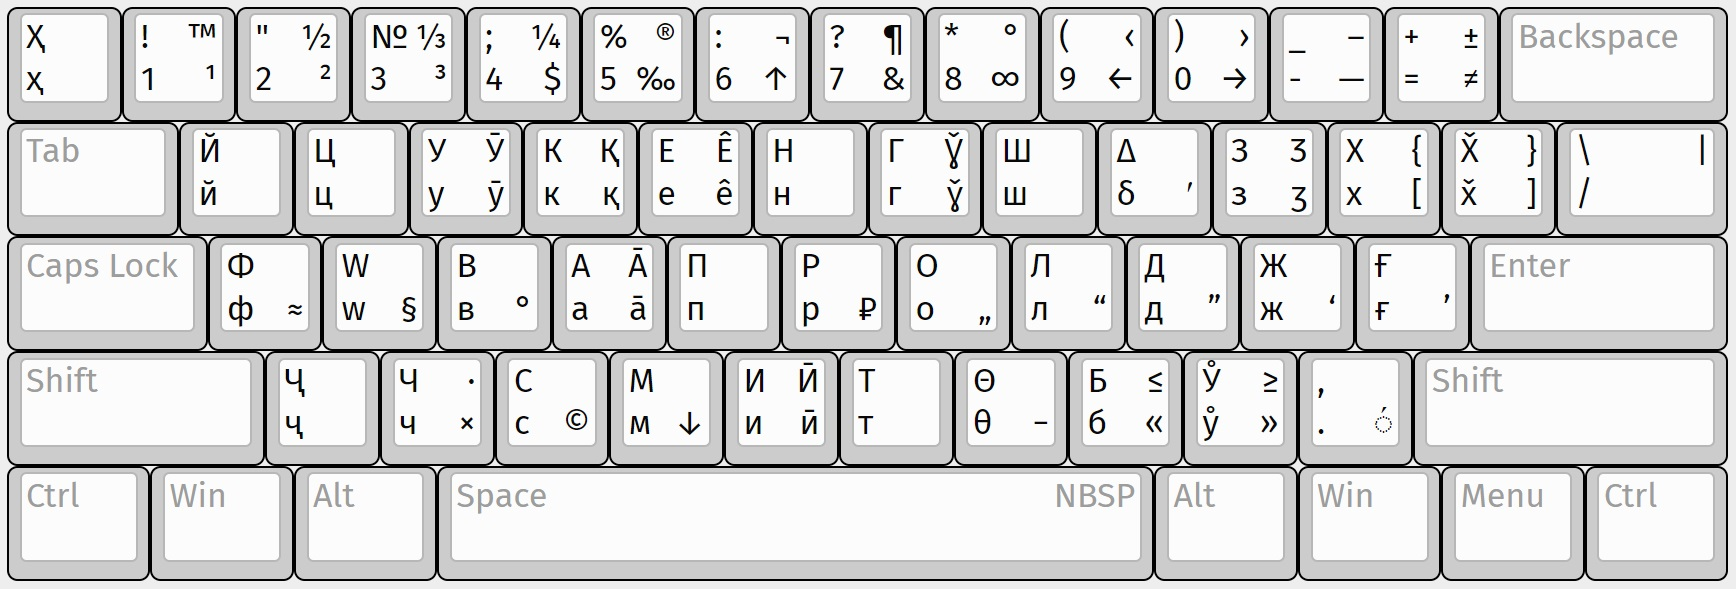
\includegraphics[width=0.8\textwidth]{img/ortho4.jpg}
\end{figure}

Наш проект — далеко не первый опыт создания шугнанской раскладки для компьютеров. К сожалению, в большинстве случаев создаваемые энтузиастами раскладки~не~отличаются удобством и~лёгкостью использования, а кроме того, отражают личные взгляды их~создателей на идеальное устройство шугнанского алфавита, которые только усугубляют проблему разнообразия письменностей. Пример такой раскладки представлен в работе \parencite[21–30]{gulomsafdarov2020}. Во-первых, в~предложенной автором раскладке для обозначения многих согласных используется диакритика «гачек» (<Т̌~т̌> /θ/, <В̌~в̌> /w/ и~другие), что~не~соответствует «консенсусному» алфавиту, представленному выше в~этом разделе. Во-вторых, автор разработал собственную схему расположения шугнанских букв на~клавиатуре вместо того, чтобы модифицировать схемы уже существующих раскладок для~русского или~таджикского. Это означает, что потенциальным пользователям придётся выучить абсолютно новую схему расположения букв, что~кажется мне нецелесообразным. В-третьих, некоторые буквы в~предложенной автором раскладке располагаются на~клавишах для~цифр, а значит, пользователь раскладки лишается возможности использовать цифры. По~этим и другим более мелким причинам я~считаю разработанную нами раскладку более удобной и~рекомендую использовать именно её.

\subsection{Рекомендации по использованию шрифтов} \label{ortho-fonts}

Предложенный выше алфавит и его Юникод-стандарт, на мой взгляд, оптимальны для использования как в быту, так и при профессиональной редактуре текста. При этом в некоторых случаях символы расширенной кириллицы и латиницы, как и диакритики, могут некорректно отображаться на электронных устройствах. Цельные символы Юникода имеют заранее установленное начертание, а начертание композитных букв с~диакритиками зависит от наличия репертуаров. Репертуаром в~Юникоде называется заранее прописанная разработчиками шрифта комбинация буквы и диакритики. Создавая репертуар, разработчики шрифтов указывают, в~каком месте диакритика будет располагаться относительно буквы. Однако разработчики многих шрифтов прописывают репертуары только для самых частых композитов — например, только для композитов с~латинскими буквами. Поэтому при использовании композитов с~кириллическими буквами диакритика может «съезжать» — это связано с~тем, что разработчики не прописали для этой комбинации репертуар, и~тогда диакритика устанавливается в «дефолтном» положении. В~Таблице \ref{tab:ortho3} на~примере буквы <Ê~ê> показано, как отличается отображение цельного символа (слева) и композита (справа) в некоторых известных шрифтах. Можно увидеть, что шрифты Fira Sans и Charis SIL поддерживают кириллические репертуары правильно, а~у~шрифтов Arial и~Times New Roman диакритика «съезжает», если буква записана композитом.

\begin{table}[h]
 \centering
 \caption{Сравнение отображения цельных символов и композитов в~разных шрифтах}
 \smallskip
 \label{tab:ortho3}
 \begin{tabular}{c|cc} \toprule
 шрифт & \makecell{латинская\\«e~с~циркумфлексом»} & \makecell{кириллическая\\«е» + циркумфлекс} \\ \midrule
 {\fontspec{FiraSans-Regular.ttf}Fira Sans} & {\fontspec{FiraSans-Regular.ttf}\large Ê~ê} & {\fontspec{FiraSans-Regular.ttf}\large Е̂~е̂} \\
 {\fontspec{Charis SIL}Charis SIL} & {\fontspec{Charis SIL}\large Ê~ê} & {\fontspec{Charis SIL}\large Е̂~е̂} \\
 {\fontspec{arial.ttf}Arial} & {\fontspec{arial.ttf}\large Ê~ê} & {\fontspec{arial.ttf}\large Е̂~е̂} \\
 {\fontspec{times.ttf}Times New Roman} & {\fontspec{times.ttf}\large Ê~ê} & {\fontspec{times.ttf}\large Е̂~е̂} \\ \bottomrule
 \end{tabular}
\end{table}

\begin{table}[ht]
 \centering
 \caption{Сравнение корректности отображения шугнанских букв с~диакритиками в~разных шрифтах (пример из словарной статьи \i{кур-кур} ‘шорох, шум’ \parencite{karamshoev1991})}
 \smallskip
 \label{tab:ortho4}
 \begin{tabular}{c|l} \toprule
 шрифт & \makecell[l]{пример отображения символов} \\ \midrule
 {\fontspec{arial.ttf}Arial} & \makecell[l]{{\fontspec{arial.ttf}Wāδ пӯрген-ен ас wи ку̊ɣ̌ӡ-ат,} \\ {\fontspec{arial.ttf}~~~каwӣҷ-инд нах̌тойд.}} \\
 {\fontspec{ARIALUNI.ttf}Arial Unicode MS} & \makecell[l]{{\fontspec{ARIALUNI.ttf}Wāδ пӯрген-ен ас wи ку̊ɣ̌ӡ-ат,} \\ {\fontspec{ARIALUNI.ttf}~~~каwӣҷ-инд нах̌тойд.}} \\
 {\fontspec{times.ttf}Times New Roman} & \makecell[l]{{\fontspec{times.ttf}Wāδ пӯрген-ен ас wи ку̊ɣ̌ӡ-ат,} \\ {\fontspec{times.ttf}~~~каwӣҷ-инд нах̌тойд.}} \\
 {\fontspec{Doulos SIL}Doulos SIL} & \makecell[l]{{\fontspec{Doulos SIL}Wāδ пӯрген-ен ас wи ку̊ɣ̌ӡ-ат,} \\ {\fontspec{Doulos SIL}~~~каwӣҷ-инд нах̌тойд.}} \\
 {\fontspec{calibri.ttf}Calibri} & \makecell[l]{{\fontspec{calibri.ttf}Wāδ пӯрген-ен ас wи ку̊ɣ̌ӡ-ат,} \\ {\fontspec{calibri.ttf}~~~каwӣҷ-инд нах̌тойд.}} \\
 {\fontspec{cambria.ttc}Cambria} & \makecell[l]{{\fontspec{cambria.ttc}Wāδ пӯрген-ен ас wи ку̊ɣ̌ӡ-ат,} \\ {\fontspec{cambria.ttc}~~~каwӣҷ-инд нах̌тойд.}} \\
 {\fontspec{CharisSIL-Regular.ttf}Charis SIL} & \makecell[l]{{\fontspec{CharisSIL-Regular.ttf}Wāδ пӯрген-ен ас wи ку̊ɣ̌ӡ-ат,} \\ {\fontspec{CharisSIL-Regular.ttf}~~~каwӣҷ-инд нах̌тойд.}} \\
 {\fontspec{FiraSans-Regular.ttf}Fira Sans} & \makecell[l]{{\fontspec{FiraSans-Regular.ttf}Wāδ пӯрген-ен ас wи ку̊ɣ̌ӡ-ат,} \\ {\fontspec{FiraSans-Regular.ttf}~~~каwӣҷ-инд нах̌тойд.}} \\
 {\fontspec{GentiumBookPlus-Regular.ttf}Gentium Book Plus} & \makecell[l]{{\fontspec{GentiumBookPlus-Regular.ttf}Wāδ пӯрген-ен ас wи ку̊ɣ̌ӡ-ат,} \\  {\fontspec{GentiumBookPlus-Regular.ttf}~~~каwӣҷ-инд нах̌тойд.}} \\
 {\fontspec{helvetica_regular.otf}Helvetica} & \makecell[l]{{\fontspec{helvetica_regular.otf}Wāδ пӯрген-ен ас wи ку̊ɣ̌ӡ-ат,} \\ {\fontspec{helvetica_regular.otf}~~~каwӣҷ-инд нах̌тойд.}} \\
 {\fontspec{Noto Sans}Noto Sans} & \makecell[l]{{\fontspec{Noto Sans}Wāδ пӯрген-ен ас wи ку̊ɣ̌ӡ-ат,} \\ {\fontspec{Noto Sans}~~~каwӣҷ-инд нах̌тойд.}} \\ 
 Noto Serif & \makecell[l]{Wāδ пӯрген-ен ас wи ку̊ɣ̌ӡ-ат, \\ ~~~каwӣҷ-инд нах̌тойд.} \\
 {\fontspec{Roboto-Regular.ttf}Roboto} & \makecell[l]{{\fontspec{Roboto-Regular.ttf}Wāδ пӯрген-ен ас wи ку̊ɣ̌ӡ-ат,} \\  {\fontspec{Roboto-Regular.ttf}~~~каwӣҷ-инд нах̌тойд.}} \\
 {\fontspec{Trebuchet MS}Trebuchet MS} & \makecell[l]{{\fontspec{Trebuchet MS}Wāδ пӯрген-ен ас wи ку̊ɣ̌ӡ-ат,} \\ {\fontspec{Trebuchet MS}~~~каwӣҷ-инд нах̌тойд.}} \\ \bottomrule
 \end{tabular}
\end{table}

Это одна из причин, по которой предпочтительно использовать цельные символы. К примеру, буква <Ê~ê> в стандартизированном алфавите, который я предложил в \hyperref[ortho-project]{Разделе~2.2}, кодируется цельным символом, и поэтому диакритика не съезжает. Однако, к сожалению, не~для~всех предложенных букв с диакритиками в Юникоде есть цельные символы. Буквы <У̊~у̊>, <Х̌~х̌> и <Ɣ̌~ɣ̌> нельзя записать цельно, поэтому для~них мы используем композиты, а они могут некорректно отображаться в некоторых шрифтах. Как можно увидеть в~Таблице \ref{tab:ortho4} ниже, в шрифтах Arial и Times New Roman диакритика расположена некорректно у двух букв: <У̊~у̊> и <Х̌~х̌>. В некоторых шрифтах встречается и~более серьёзная проблема: в шрифте нет даже самого начертания определённых символов, и в современных программах такие символы автоматически отображаются с помощью другого шрифта. К примеру, как~показано в~Таблице \ref{tab:ortho4}, в~шрифте Trebuchet MS нет многих символов шугнанской кириллицы.

Проблема некорректного отображения решается использованием шрифтов, которые поддерживают шугнанские символы. Шрифты Arial Unicode MS, Calibri, Cambria, входящие в стандартный пакет Windows, правильно отображают буквы шугнанской кириллицы. Кроме того, есть ряд подходящих шрифтов, которые распространяются по свободной лицензии (их можно найти и бесплатно скачать в интернете): это Andika, Charis SIL, DejaVu Sans, DejaVu Serif, Doulos SIL, Fira Sans, Gentium Plus, New CM Sans, New CM Serif и Noto Sans.

Для~многих популярных шрифтов, неправильно отображающих шугнанские символы, можно найти более подходящие аналоги. Так,~вместо Times New Roman можно пользоваться бесплатным шрифтом Doulos SIL, который визуально похож на~Times New Roman. Вместо стандартного Arial можно пользоваться его расширенной версией Arial Unicode MS (см.~Таблицу \ref{tab:ortho4}).

\begin{figure}[ht]
 \centering 
 \caption{Сравнение отображения таджикского текста из учебника Аламшоева [\cite*[4]{alamshoev2014}] в~«таджикском» шрифте Times New Roman Tj и обычном Times New Roman}
 \smallskip
 \label{fig:ortho5}

 \begin{quote} \begin{spacing}{1.2}
 \b{Times New Roman Tj}: {\fontspec{Times_New_Roman_Tj.ttf}Ин дастур, ки ба курси шунавандагони забони шуѓнонї, яке аз ќадимтарин забонњои эронї бахшида шудааст, барои хубтар аз худ кардани ин забон пешбинї шудааст. Дастур асосан барои хонандагони тољикзабон, ки мехоњанд забони шуѓнониро аз худ кунанд, тартиб дода шудааст. Пеш аз њама муаллим бояд ба шунавандагон дар бораи  таърихи пайдоиши забонњои эронї ва алалхусус, гурўњи шарќии он — забонњои помирї маълумот дињад.}
 \end{spacing} \end{quote}

 \begin{quote} \begin{spacing}{1.2}
 \b{Times New Roman}: {\fontspec{times.ttf}Ин дастур, ки ба курси шунавандагони забони шуѓнонї, яке аз ќадимтарин забонњои эронї бахшида шудааст, барои хубтар аз худ кардани ин забон пешбинї шудааст. Дастур асосан барои хонандагони тољикзабон, ки мехоњанд забони шуѓнониро аз худ кунанд, тартиб дода шудааст. Пеш аз њама муаллим бояд ба шунавандагон дар бораи  таърихи пайдоиши забонњои эронї ва алалхусус, гурўњи шарќии он — забонњои помирї маълумот дињад.}
 \end{spacing} \end{quote}
\end{figure}

\pagebreak[3]

Наконец, стоит обратиться к такому явлению, как «таджикские шрифты». Это модифицированные версии известных шрифтов, в~которых вместо дополнительных символов таджикской кириллицы используются другие символы, но они отображаются как~таджикские буквы (см.~Рисунок~\ref{fig:ortho5}). Например, буква, которая в одном из самых употребительных «таджикских шрифтов» Times New Roman Tj выглядит как <Ҳ~ҳ>, на самом деле кодируется символом для буквы из~сербского алфавита <Њ~њ>. По-видимому, создание таких кустарных инструментов для работы с текстом приходится на 1990-е годов, когда~распространённые компьютерные шрифты не~поддерживали буквы таджикского алфавита \parencite{graschenko2011}. В~настоящее время буквы как~таджикского, так~и~шугнанского алфавитов поддерживаются огромным количеством шрифтов, и~необходимости в~«таджикских шрифтах»-обманках нет. Однако они всё ещё активно используются в работе как с таджикским, так~и с~шугнанским языком. К~примеру, учебник Аламшоева [\cite*{alamshoev2014}], по-видимому, был напечатан с~помощью Times New Roman Tj.

Я не рекомендую использовать «таджикские шрифты» для~работы с~шугнанскими (как и с таджикскими) текстами. Набранный таким образом текст будет корректно отображаться только в Microsoft Word (или~аналогичных редакторах), но~при копировании текста в~другие программы, где~выбор «таджикских шрифтов» недоступен (например, в~веб-браузер) или~при~открытии на~устройстве, где не установлен нужный шрифт, он~станет нечитаемым (см.~Рисунок~\ref{fig:ortho5}).

С~помощью инструментов, представленных в статье (в частности, с~помощью раскладок для~компьютеров и~рекомендованных шрифтов), любой пользователь компьютеров на~Windows или macOS сможет быстро и~удобно печатать аккуратно выглядящие тексты на~шугнанском языке, не~прибегая к~самостоятельному поиску символов,~«таджикским шрифтам» или~другим сложным техническим находкам.